\section{Results}
In this section, results from silulations made with the final version of the software are presented. Plots are included when it has been considered as important to show how a property has developed during the simulations. The simulation setups are explained in the Simulations section of this report. For an analys and discussion of the result, se Analysis section.
\subsection{Energies}
Plots of the potential, kinetic and total energy are displayed to show that equilibrium is reached. 
\subsubsection{Total energy}
The total energy had an average value of -9886.78 eV for this setup and showed a fluctruation of at most 0.1\% of the average value (see plot in \ref{totale}).
\begin{figure}[h]
	\centering
	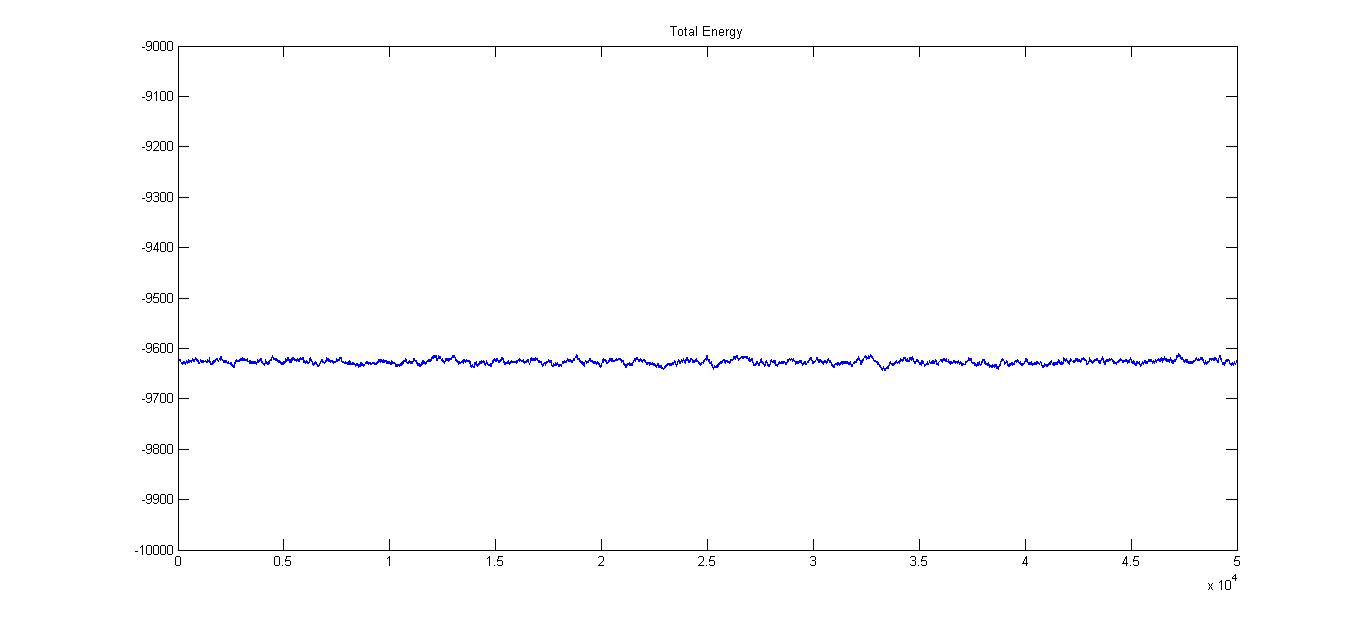
\includegraphics[width=1\textwidth]{total1.jpg}
	\caption{Plotted values of the kinetic energy over 50000 timesteps.}
	\label{totale}
\end{figure}

\subsubsection{Kinetic energy}
The kinetic energy reached an average value of 258.73 eV and had a maximum fluctruation of 5\% from the average value (see plot in \ref{kinetic}).
\begin{figure}[h]
	\centering
	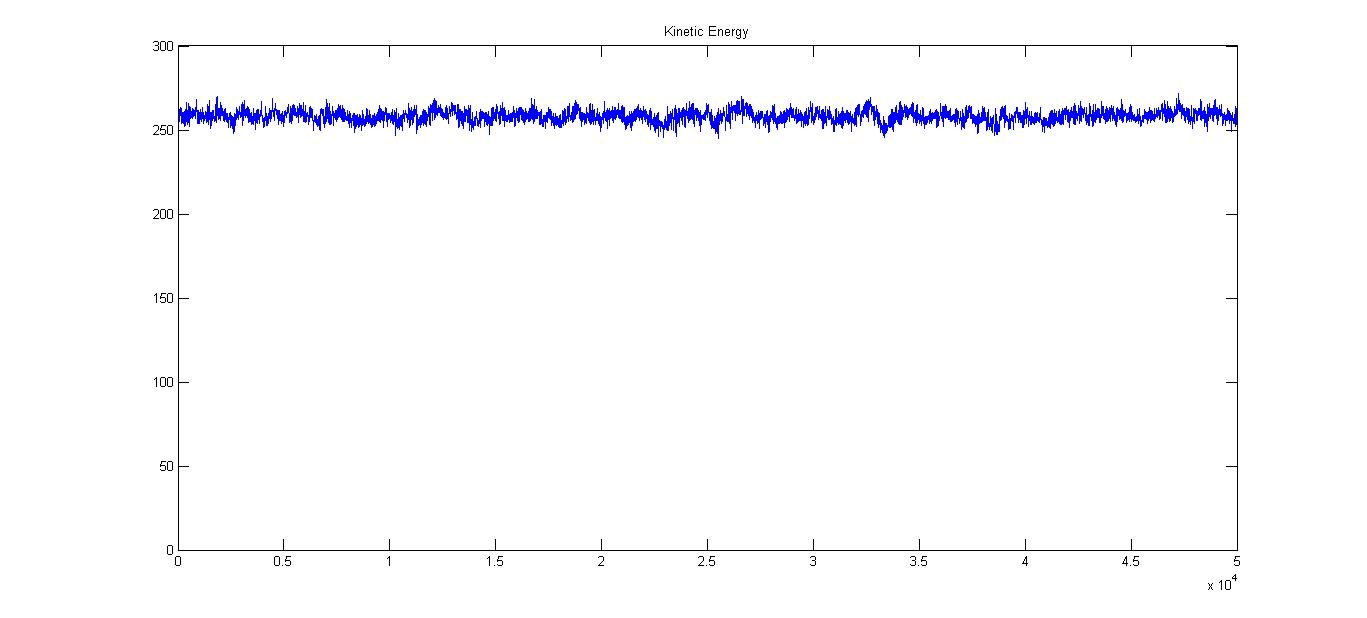
\includegraphics[width=1\textwidth]{kinetic.jpg}
	\caption{Plotted values of the kinetic energy over 50000 timesteps.}
	\label{kinetic}
\end{figure}

\subsubsection{Potential energy}
\subsubsection{Cohesive energy}
\subsection{Temperature}
\subsection{MSD}
\subsection{Internal pressure}
\subsection{Debye Temperature}
\subsection{Specific heat}
\subsection{Diffusion coefficient}
\subsection{Reaching equilibrium}
